\subsection{\underline{OLSR}}
    \textit{OLSR} est un protocole proactif à état de liens. Il fournit un support à certaines extensions comme
    sleep mode operation, multicast-routing etc.\\
    Ce protocole utilise deux types de messages:\\
    \begin{enumerate}
        \item \textit{hello}\\
            Ces paquets sont envoyés à un saut. Ils sont utilisés pour constituer le voisinage et
            l'ensemble des \textit{"multipoint relays" (MPR)}. (concept expliqué  \hyperlink{mpr}{ici})\\
            Ils contiennent le statut des liens d'un noeud avec tout son voisinage.
        \item \textit{topology control (TC)}\\
            Diffusés dans tous le réseau par les \textit{MPR}. Ils contiennent la liste de tous les \textit{MPRs}
            du noeud qui émet ce paquet.
    \end{enumerate}
    \hypertarget{mpr}{\textit{\textbf{MPR}}}\\
    Les multipoint relays sont des noeuds qui sont chargés d'effectuer le broadcasting des \textit{TCs}. \\
    L'ensemble des \textit{MPRs} d'un réseau \textit{OLSR} forme un arbre couvrant du réseau. Trouver ce sous-ensemble de sommets
    est un problème \textit{NP-Complet}. \textit{DSR} propose une heuristique simple pour calculer cet ensemble de \textit{MPRs}.\\
    
    \begin{figure}[H]
        \centering
        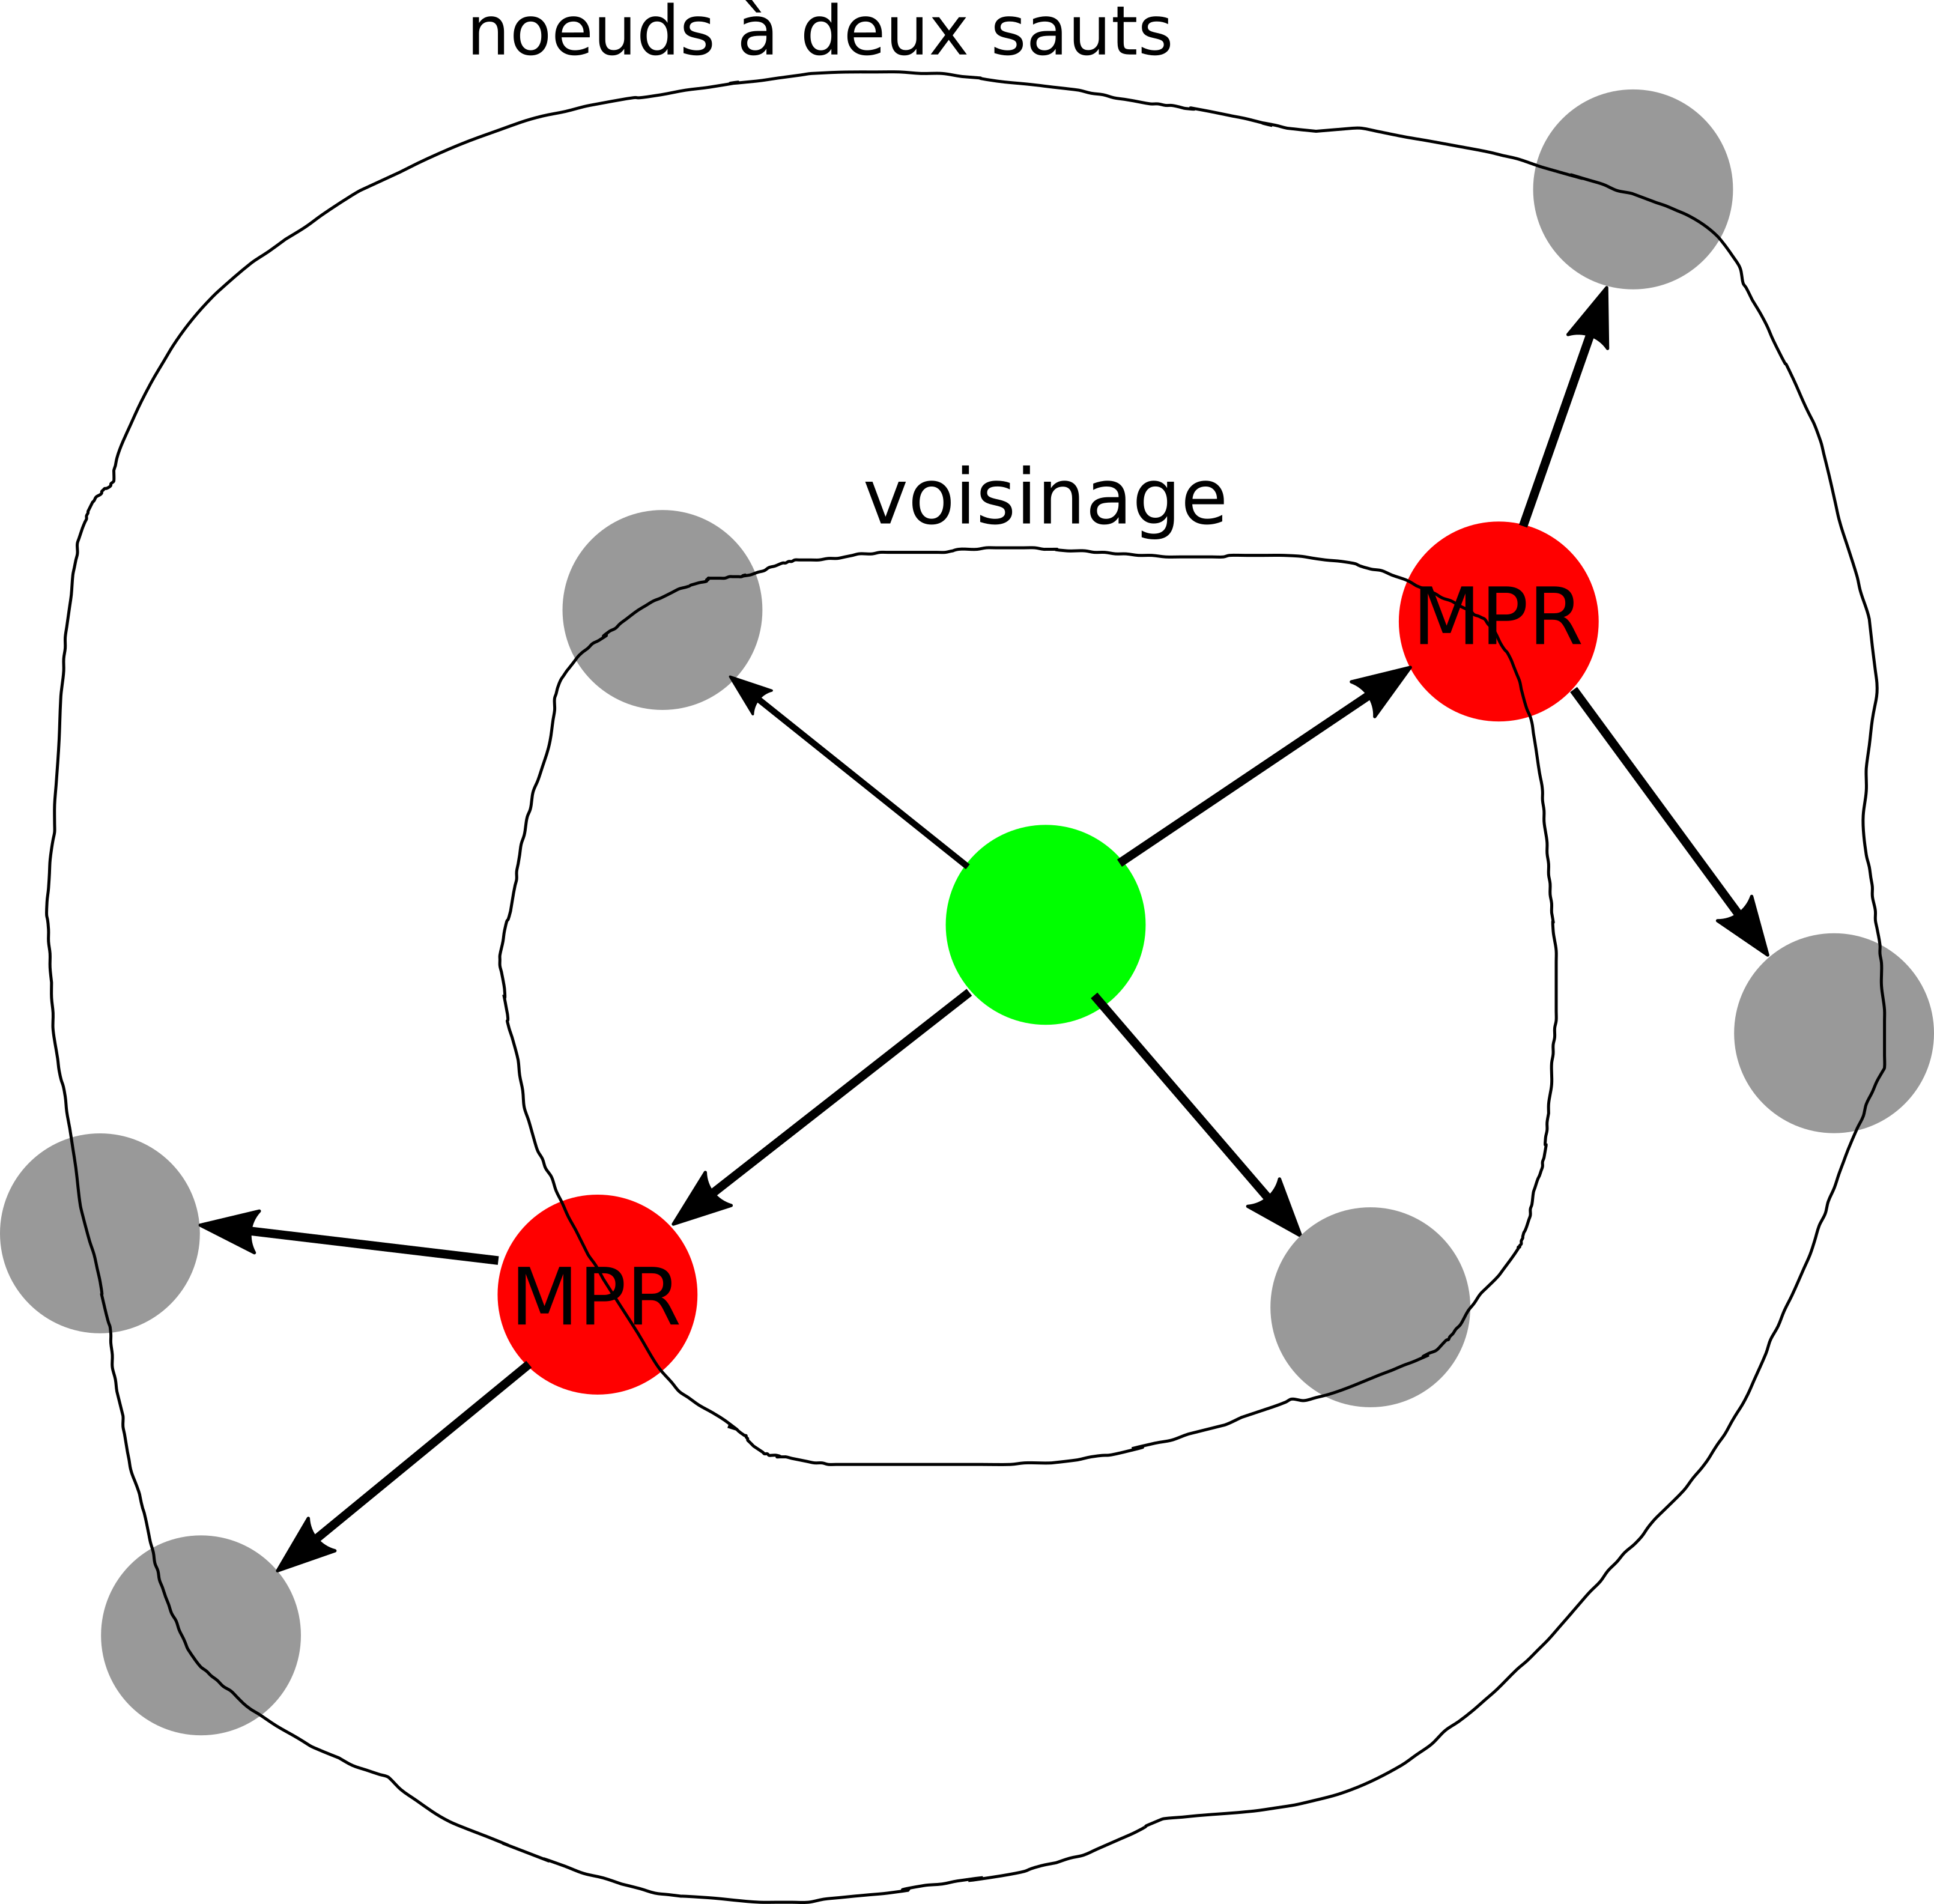
\includegraphics[scale=0.5]{images/olsr.png}
        \caption{Shéma d'un réseau OLSR}
        \label{olsr}
    \end{figure}
    \textbf{Découverte de voisins}\\
    La découverte de voisins se fait comme suit:
    \begin{itemize}
        \item Quand un noeud B reçoit un message \textit{hello} d'un noeud A,
            il va rajouter A dans ses voisins avec le statut asymétrique
        \item B va ensuite envoyer un message \textit{hello} avec A asymétrique dans la liste de voisins.
        \item Quand A reçoit ce message, il va pouvoir modifier le statut de B à symétrique.
        \item A renvoie un message \textit{hello} avec B symétrique dans la liste des voisins.
        \item Quand B reçoit ce message il modifie le statut de A à symétrique
    \end{itemize}
    \begin{figure}[H]
        \centering
        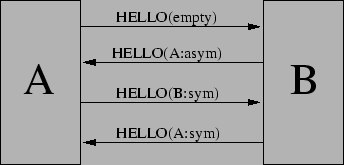
\includegraphics[scale=0.6]{images/olsr_neighborDiscovery.png}
        \caption{découverte de voisins en utilisant les messages \textit{hello} \cite{olsr_neighborDiscovery_w}}
        \label{olsr_neighborDiscovery}
    \end{figure}